% 第1章第5节：轨迹计算中的误差传播（初值与逐步计算误差；输入与模型扰动）。

\section{轨迹计算中的误差传播}
\label{sec:dds-error-propagation}

上一节看到，有限精度可以让$r=4$的Logistic轨道在五十步内完全失真。本节把这种现象放进一般框架：离散模型已经给定，我们实际算出的序列与模型的真实轨道相差多少？误差有几个来源：初值不准，每一步计算带有残差，输入与设定值有偏差，模型本身与要描述的过程有出入。它们注入的位置不同，却都要经过此后的动力学传播。

需要说明比较的对象。这里递推本身就是模型，我们问的是“这个递推算得多准”。第~\ref{chap:ordinary-differential-equations}章用离散步长逼近常微分方程时，递推是对另一个连续对象的近似，误差还包括每步的截断误差，即离散公式与连续演化之差。两种误差在数学上可以用同一个累计不等式处理，但来源和随步长变化的方式不同，不应混为一谈。

\subsection{初值与逐步计算误差}
\label{sec:dds-computation-error}

\paragraph{把计算误差写成每步残差}
设模型为$\bm x_{n+1}=F(\bm x_n)$，实际算出的序列为$\hat{\bm x}_n$。无论误差来自舍入、内层迭代没有完全收敛，还是用查表或低精度近似代替了$F$，都可以统一写成
\[
  \hat{\bm x}_{n+1}=F(\hat{\bm x}_n)+\bm r_n ,
\]
其中$\bm r_n$是第$n$步的残差：把上一步的计算值代入模型，与本步计算值的差。记误差$\bm e_n=\hat{\bm x}_n-\bm x_n$。若$F$在某个区域$D$上满足$\lVert F(\bm x)-F(\bm y)\rVert\leq L\lVert\bm x-\bm y\rVert$，且两条序列都在$D$中，则
\[
  \lVert\bm e_{n+1}\rVert\leq\lVert F(\hat{\bm x}_n)-F(\bm x_n)\rVert+\lVert\bm r_n\rVert\leq L\lVert\bm e_n\rVert+\lVert\bm r_n\rVert .
\]
误差满足一个“乘以$L$、再加新残差”的标量不等式。它的解与第~\ref{sec:dds-constant-coefficient}小节的仿射递推有同样的结构。

\begin{lemma}[离散Grönwall不等式]
\label{lem:dds-discrete-gronwall}
设非负数列$(a_n)$、$(b_n)$、$(L_n)$满足$a_{n+1}\leq L_na_n+b_n$，$n\geq0$。则
\[
  a_n\leq\Bigl(\prod_{k=0}^{n-1}L_k\Bigr)a_0+\sum_{k=0}^{n-1}\Bigl(\prod_{i=k+1}^{n-1}L_i\Bigr)b_k ,
\]
空乘积取$1$。特别地，$L_n\equiv L$时$a_n\leq L^na_0+\sum_{k=0}^{n-1}L^{\,n-1-k}b_k$。
\end{lemma}

\begin{proof}
$n=0$时右边为$a_0$。若对$n$成立，则因$L_n\geq0$，
\[
  a_{n+1}\leq L_na_n+b_n\leq\Bigl(\prod_{k=0}^{n}L_k\Bigr)a_0+\sum_{k=0}^{n-1}\Bigl(\prod_{i=k+1}^{n}L_i\Bigr)b_k+b_n ,
\]
最后一项正是$k=n$时的求和项。
\end{proof}

引理与递推解~\eqref{eq:dds-variation-constants}一一对应：初始误差像初态一样被逐步放大或缩小，每步残差像输入一样在注入后继续传播。只是这里用不等式代替了等式，用Lipschitz常数代替了矩阵。

\begin{theorem}[逐步计算误差的传播界]
\label{thm:dds-error-propagation}
设$D\subseteq\mathbb R^d$，$F:D\to\mathbb R^d$在$D$上$L$-Lipschitz。设模型轨道$\bm x_{n+1}=F(\bm x_n)$与计算序列$\hat{\bm x}_{n+1}=F(\hat{\bm x}_n)+\bm r_n$在$0\leq n\leq N$时都位于$D$中，且$\lVert\bm r_n\rVert\leq\eta$。则对$0\leq n\leq N$，
\begin{equation}
  \lVert\hat{\bm x}_n-\bm x_n\rVert\leq L^n\lVert\hat{\bm x}_0-\bm x_0\rVert+\eta\sum_{k=0}^{n-1}L^k
  =\begin{cases}
    L^n\lVert\hat{\bm x}_0-\bm x_0\rVert+\eta\dfrac{L^n-1}{L-1},&L\neq1,\\[1ex]
    \lVert\hat{\bm x}_0-\bm x_0\rVert+n\eta,&L=1.
  \end{cases}
  \label{eq:dds-error-propagation}
\end{equation}
\end{theorem}

\begin{proof}
前面已得$\lVert\bm e_{n+1}\rVert\leq L\lVert\bm e_n\rVert+\eta$，对$a_n=\lVert\bm e_n\rVert$、$L_n=L$、$b_n=\eta$用引理~\ref{lem:dds-discrete-gronwall}。
\end{proof}

上界分成三种情形，对应三种截然不同的计算体验。$L<1$时，初始误差几何衰减，残差的累计被几何级数封顶，$\limsup_n\lVert\bm e_n\rVert\leq\eta/(1-L)$：误差不会越积越多。$L=1$时，残差线性累计，长时间计算的误差随步数增长。$L>1$时，误差可能按$L^n$增长，有限时间内可控，长时间则无界。定理的前提“两条序列都在$D$中”需要单独核实：若误差把计算序列推出了Lipschitz估计成立的区域，上界就不再适用，这在$L>1$时尤其要注意。

图~\ref{fig:dds-error-bound}用两个例子对比上界与实际误差。(a)中$F=\cos$，初值误差$0.1$，每步人为加入幅度不超过$\eta=10^{-3}$的残差；轨道在$[0,1.01]$中，取$L=0.85\geq\sin1.01$。实际误差很快降到$10^{-3}$量级并在其中起伏，上界从$0.1$平滑地降到$\eta/(1-L)\approx6.7\times10^{-3}$，始终在实际误差之上。(b)中$F(x)=4x(1-x)$用双精度计算，每步舍入残差不超过$2^{-52}\approx2.2\times10^{-16}$，$[0,1]$上的Lipschitz常数是$\max|F'|=4$。上界按$4^n$增长，实际误差却大致按$2^n$增长。

\begin{figure}[htbp]
  \centering
  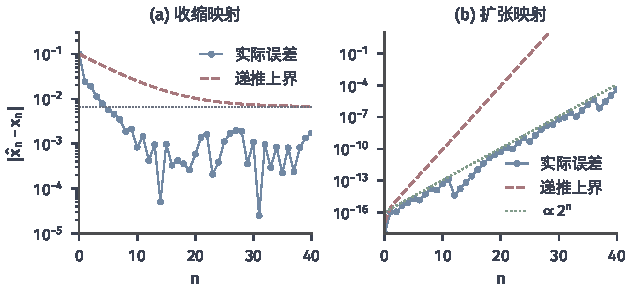
\includegraphics[width=107mm]{figures/03-optimization-evolution-and-signals/02-processes-and-trajectory-evolution/matplotlib/dds-error-bound/figure.pdf}
  \caption{递推误差上界与实际误差，纵轴取对数。(a)收缩映射$\cos x$：真实轨道从$0.2$出发，计算序列从$0.3$出发且每步加入幅度在$[\eta/2,\eta]$、符号随机（固定种子）的残差，$\eta=10^{-3}$；红色虚线为式~\eqref{eq:dds-error-propagation}取$L=0.85$的上界，点线为其极限$\eta/(1-L)$。(b)扩张映射$4x(1-x)$：双精度计算与$120$位参考轨道之差，上界取$L=4$、每步残差$2^{-52}$，并计入$0.2$的初始表示误差；绿色点线示意$2^n$的增长。}
  \label{fig:dds-error-bound}
\end{figure}

(b)中的差距说明了Lipschitz上界的保守之处。$L=4$是$|F'|$在整个区间上的最大值，只在$x=0$与$x=1$附近取到；一条典型轨道各处都要经过，它感受到的是沿轨道导数的几何平均，即第~\ref{sec:dds-sensitivity}小节的Lyapunov指数$\ln2$。若把引理中的常数$L$换成沿轨道的局部放大因子$L_k\approx|F'(x_k)|$，就能得到贴近实际的估计，代价是这些因子依赖具体轨道，事先不知道。

\paragraph{收缩更新的长期残差界}
收缩情形最值得在实际计算中利用。设$F$在完备的正向不变集$D$上是$L$-压缩（$L<1$），不动点为$\bm x_*$。以$\bm x_0=\bm x_*$为模型轨道代入定理~\ref{thm:dds-error-propagation}（仍需假设计算序列留在$D$中），得到
\[
  \lVert\hat{\bm x}_n-\bm x_*\rVert\leq L^n\lVert\hat{\bm x}_0-\bm x_*\rVert+\frac{\eta}{1-L}.
\]
无论迭代多久，计算精度都被$\eta/(1-L)$兜住；反过来，要把不动点算到精度$\varepsilon$，每步残差必须小于$(1-L)\varepsilon$。$L$越接近$1$，收缩越弱，对每步精度的要求越苛刻，这是压缩映射的一种“条件数”。

事后估计用已经算出的量判断离不动点有多远。由$\hat{\bm x}_n-\bm x_*=(\hat{\bm x}_n-F(\hat{\bm x}_n))+(F(\hat{\bm x}_n)-F(\bm x_*))$与三角不等式，
\[
  \lVert\hat{\bm x}_n-\bm x_*\rVert\leq\lVert F(\hat{\bm x}_n)-\hat{\bm x}_n\rVert+L\lVert\hat{\bm x}_n-\bm x_*\rVert ,
\]
移项后再用$F(\hat{\bm x}_n)=\hat{\bm x}_{n+1}-\bm r_n$，
\begin{equation}
  \lVert\hat{\bm x}_n-\bm x_*\rVert\leq\frac{\lVert F(\hat{\bm x}_n)-\hat{\bm x}_n\rVert}{1-L}\leq\frac{\lVert\hat{\bm x}_{n+1}-\hat{\bm x}_n\rVert+\eta}{1-L}.
  \label{eq:dds-a-posteriori}
\end{equation}
所以“相邻两步很接近就停止”在收缩映射下是有依据的，但要乘上因子$1/(1-L)$，还要计入残差$\eta$：步长小于$10^{-8}$、$L=0.99$时，离不动点的距离只能保证小于约$10^{-6}$。

\paragraph{相邻两步很近不等于接近极限}
没有收缩条件，步长小就说明不了什么。$x_{n+1}=x_n+1/x_n$从$x_0=1$出发，第$10^4$步的步长约为$0.007$，第$10^5$步约为$0.0022$，越来越小，轨道却按$\sqrt{2n}$的速度趋于无穷：步长趋于零，序列不收敛。即使序列确实收敛，步长也可能严重低估距离。回到$x_{n+1}=x_n-x_n^3$，$x_0=0.5$时第$1000$步的步长$x_n^3\approx1.1\times10^{-5}$，离极限$0$的距离却是$0.022$，是步长的两千倍。原因是原点处导数为$1$，收缩因子趋于$1$，式~\eqref{eq:dds-a-posteriori}中的$1/(1-L)$趋于无穷。判断“已经接近极限”需要动力学条件与残差一起提供依据。

\paragraph{不稳定更新放大微小残差}
误差放大最直观的例子，是试图沿着不稳定的平衡点做长时间计算。

\begin{example}[从不稳定平衡点出发的浮点计算]
\label{ex:dds-unstable-fixed-point}
取$r=3.3$的Logistic映射，平衡点$x_r=1-1/3.3=0.69\overline{69}$，这里$F'(x_r)=2-3.3=-1.3$，平衡点不稳定。把双精度下最接近$x_r$的数作为初值，第一步的残差只有约$2.2\times10^{-16}$，此后偏差每步约乘以$1.3$：第$50$步约$10^{-10}$，第$100$步约$5\times10^{-5}$，第$131$步超过$0.1$，计算序列离开平衡点，转向稳定的周期二轨道。模型轨道一动不动，计算轨道却在一百多步后面目全非。在不稳定的方向上，再小的残差也会被持续放大，这与上一节$r=4$的现象同源。
\end{example}

\subsection{输入与模型扰动}
\label{sec:dds-input-model-perturbation}

\paragraph{线性系统中的输入扰动}
初值误差只在开始时注入一次，输入误差却可能在每一步都注入。设两组初值和输入$(\bm x_0,\bm u)$与$(\tilde{\bm x}_0,\tilde{\bm u})$驱动同一个系统$\bm x_{n+1}=\bm A\bm x_n+\bm B\bm u_n$。两条轨道之差$\bm\delta_n=\bm x_n-\tilde{\bm x}_n$满足同一个线性递推，输入换成$\bm u_n-\tilde{\bm u}_n$，所以由式~\eqref{eq:dds-variation-constants}，
\[
  \bm\delta_n=\bm A^n\bm\delta_0+\sum_{j=0}^{n-1}\bm A^{\,n-1-j}\bm B(\bm u_j-\tilde{\bm u}_j).
\]

\begin{theorem}[稳定线性系统的输入响应界]
\label{thm:dds-input-response}
设$\lVert\bm A^k\rVert\leq Cq^k$对全部$k\geq0$成立，$C\geq1$，$0\leq q<1$（由定理~\ref{thm:dds-spectral-stability}，$\rho(\bm A)<1$时这样的$C,q$存在）。则
\begin{equation}
  \lVert\bm\delta_n\rVert\leq Cq^n\lVert\bm\delta_0\rVert+C\lVert\bm B\rVert\sum_{j=0}^{n-1}q^{\,n-1-j}\lVert\bm u_j-\tilde{\bm u}_j\rVert .
  \label{eq:dds-input-response}
\end{equation}
特别地：
\begin{enumerate}
  \item 若$\sup_j\lVert\bm u_j-\tilde{\bm u}_j\rVert\leq U$，则$\lVert\bm\delta_n\rVert\leq Cq^n\lVert\bm\delta_0\rVert+C\lVert\bm B\rVert U/(1-q)$对全部$n$成立；
  \item 若$\lVert\bm u_j-\tilde{\bm u}_j\rVert\to0$，则$\bm\delta_n\to\bm0$。
\end{enumerate}
\end{theorem}

\begin{proof}
式~\eqref{eq:dds-input-response}由三角不等式与$\lVert\bm A^k\bm B\bm v\rVert\leq Cq^k\lVert\bm B\rVert\lVert\bm v\rVert$得到；(1)再用$\sum_{k\geq0}q^k=1/(1-q)$。对(2)，记$w_j=\lVert\bm u_j-\tilde{\bm u}_j\rVert$，它有界，设上界为$W$。给定$\varepsilon>0$，取$J$使$j\geq J$时$w_j<\varepsilon$。把求和拆成$j<J$与$j\geq J$两段：
\[
  \sum_{j=0}^{n-1}q^{\,n-1-j}w_j\leq W\sum_{j<J}q^{\,n-1-j}+\varepsilon\sum_{j\geq J}q^{\,n-1-j}\leq Wq^{\,n-J}\frac{1}{1-q}+\frac{\varepsilon}{1-q}.
\]
$n\to\infty$时第一项趋于零，所以$\limsup_n\lVert\bm\delta_n\rVert\leq C\lVert\bm B\rVert\varepsilon/(1-q)$；$\varepsilon$任意，得$\bm\delta_n\to\bm0$。
\end{proof}

定理把输入扰动的影响分成两类。有界扰动产生有界的状态偏差，偏差的大小由扰动幅度和系统的“记忆长度”$1/(1-q)$共同决定。会消失的扰动最终不留痕迹。但持续存在的扰动会留下持续的偏差，而不会因为系统稳定就消失：温度例中若加热量一直比设定值多$0.05$，由式~\eqref{eq:dds-forced-equilibrium}，平衡温差升高$0.05/(1-0.8)=0.25$。图~\ref{fig:dds-forced-response}比较了这两种扰动：初值都偏了$1$，持续偏差的轨道最终停在高出$0.25$的位置，衰减扰动（$0.3\cdot0.7^n$）的轨道则回到标称轨迹上。

\begin{figure}[htbp]
  \centering
  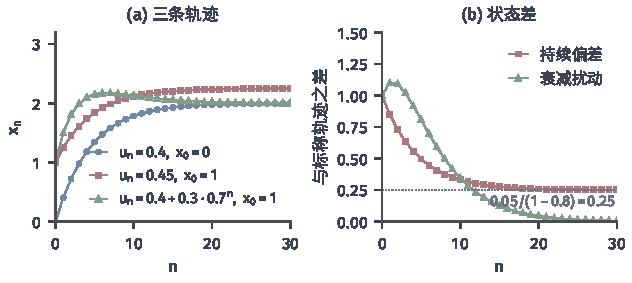
\includegraphics[width=107mm]{figures/03-optimization-evolution-and-signals/02-processes-and-trajectory-evolution/matplotlib/dds-forced-response/figure.pdf}
  \caption{持续偏差与衰减扰动。系统$x_{n+1}=0.8x_n+u_n$。(a)标称轨迹（蓝，$x_0=0$，$u_n=0.4$）、持续偏差（红，$x_0=1$，$u_n=0.45$）与衰减扰动（绿，$x_0=1$，$u_n=0.4+0.3\cdot0.7^n$）。(b)后两者与标称轨迹之差：初值差$1$按$0.8^n$消退；持续偏差留下$0.05/(1-0.8)=0.25$的稳态差（点线），衰减扰动的影响则趋于零。}
  \label{fig:dds-forced-response}
\end{figure}

稳定性是定理的必要前提。$\rho(\bm A)\geq1$时，有界输入可以产生无界状态：标量$a=1$的系统$x_n=x_0+\sum_{j<n}u_j$只是把输入累加起来，恒定的微小偏差$\delta u$也会造成线性增长的误差$n\,\delta u$。所以“初值误差会消退”与“输入误差有界”都要以稳定性为条件，而且二者分别回答不同的问题，不能用前者代替后者。

\paragraph{非线性更新中的输入与模型误差}
非线性系统没有显式解，但第~\ref{sec:dds-computation-error}小节的论证可以照搬，只需把每一步的不一致来源分开写。设真实过程按$\bm x_{n+1}=F(\bm x_n,\bm u_n)$演化，我们用另一个模型$\tilde F$和输入$\tilde{\bm u}_n$计算$\tilde{\bm x}_{n+1}=\tilde F(\tilde{\bm x}_n,\tilde{\bm u}_n)$。假设两条轨道都留在区域$D$中，并且在$D$上
\[
  \begin{gathered}
  \lVert F(\bm x,\bm u)-F(\bm y,\bm u)\rVert\leq L\lVert\bm x-\bm y\rVert,\qquad
  \lVert F(\bm x,\bm u)-F(\bm x,\bm v)\rVert\leq L_u\lVert\bm u-\bm v\rVert,\\
  \lVert F(\bm x,\bm u)-\tilde F(\bm x,\bm u)\rVert\leq\mu .
  \end{gathered}
\]
把一步差拆成三段：
\[
  \begin{aligned}
  \bm x_{n+1}-\tilde{\bm x}_{n+1}
  ={}&\bigl[F(\bm x_n,\bm u_n)-F(\tilde{\bm x}_n,\bm u_n)\bigr]
  +\bigl[F(\tilde{\bm x}_n,\bm u_n)-F(\tilde{\bm x}_n,\tilde{\bm u}_n)\bigr]\\
  &+\bigl[F(\tilde{\bm x}_n,\tilde{\bm u}_n)-\tilde F(\tilde{\bm x}_n,\tilde{\bm u}_n)\bigr],
  \end{aligned}
\]
分别对应状态差的传播、输入差和模型差。由引理~\ref{lem:dds-discrete-gronwall}，
\begin{equation}
  \lVert\bm x_n-\tilde{\bm x}_n\rVert\leq L^n\lVert\bm x_0-\tilde{\bm x}_0\rVert+\sum_{k=0}^{n-1}L^{\,n-1-k}\bigl(L_u\lVert\bm u_k-\tilde{\bm u}_k\rVert+\mu\bigr).
  \label{eq:dds-model-perturbation}
\end{equation}
三类误差来源不同，却都要经过此后的动力学传播；$L<1$时它们的累计都被几何级数封顶。

用一个数值例子说明怎样核实这些条件。

\begin{example}[线性模型代替带平方散热的温度模型]
\label{ex:dds-model-mismatch}
设房间散热还有一个与温差平方成正比的部分，真实更新为$F(x,u)=0.8x+u-0.01x^2$，而我们用线性模型$\tilde F(x,u)=0.8x+u$计算，输入都取$u_n=0.4$，初值都为$0$。先找共同的正向不变区域：在$D=[0,2]$上，$\tilde F$把$D$映到$[0.4,2]$，$F$把$D$映到$[0.4,1.96]$，都在$D$内。再算常数：$\partial_xF=0.8-0.02x\in[0.76,0.8]$，故$L=0.8$；模型差$0.01x^2\leq0.04$，故$\mu=0.04$；输入相同，第二项为零。代入式~\eqref{eq:dds-model-perturbation}，两条轨道之差不超过$0.04(1-0.8^n)/0.2<0.2$。实际上线性模型的平衡点为$2$，真实模型的平衡点满足$0.01x^2+0.2x-0.4=0$，约为$1.832$，长期差约$0.168$，确实在界内。界的大小依赖所选区域：若取更大的$D$，$\mu$会变大，界也随之变松。
\end{example}

本章到此只回答“给定的输入使状态改变了多少”。若要根据观测反过来选择输入，使状态保持在期望位置并抑制扰动的影响，就进入了控制问题，那里会把本节的输入响应界和Lyapunov函数作为设计工具重新使用。
